
\section{Simulations}


\begin{table}[H]
    \begin{center}
        \caption{Size of the test calculated for different sample sizes ($T = 250, 350, 500, 1000$) and confident levels ($\alpha = 0.01, 0.05, 0.10$)}
        \label{tab:size_nw}
        \centering
        % latex table generated in R 3.4.3 by xtable 1.8-2 package
% 
\begin{tabular}{rrrr}
  \hline
 & 0.01 & 0.05 & 0.1 \\ 
  \hline
250 & 0.015 & 0.052 & 0.095 \\ 
  350 & 0.014 & 0.059 & 0.119 \\ 
  500 & 0.007 & 0.041 & 0.101 \\ 
   \hline
\end{tabular}

    \end{center}
\end{table}

\begin{table}[H]
    \begin{center}
        \caption{Power of the test calculated for different sample sizes ($T = 250, 350, 500, 1000$) and confident levels ($\alpha = 0.01, 0.05, 0.10$) for $a = 0.25$}
        \label{tab:power_025_nw}
        \centering
        % latex table generated in R 3.4.3 by xtable 1.8-2 package
% 
\begin{tabular}{rrrr}
  \hline
 & 0.01 & 0.05 & 0.1 \\ 
  \hline
250 & 0.118 & 0.267 & 0.342 \\ 
  350 & 0.145 & 0.342 & 0.451 \\ 
  500 & 0.282 & 0.441 & 0.584 \\ 
   \hline
\end{tabular}

    \end{center}
\end{table}

\begin{table}[H]
    \begin{center}
        \caption{Power of the test calculated for different sample sizes ($T = 250, 350, 500, 1000$) and confident levels ($\alpha = 0.01, 0.05, 0.10$) for $a = 0.50$}
        \label{tab:power_050_nw}
        \centering
        % latex table generated in R 3.4.3 by xtable 1.8-2 package
% 
\begin{tabular}{rrrr}
  \hline
 & 0.01 & 0.05 & 0.1 \\ 
  \hline
250 & 0.681 & 0.795 & 0.874 \\ 
  350 & 0.839 & 0.941 & 0.961 \\ 
  500 & 0.964 & 0.987 & 0.993 \\ 
   \hline
\end{tabular}

    \end{center}
\end{table}

\begin{table}[H]
    \begin{center}
        \caption{Power of the test calculated for different sample sizes ($T = 250, 350, 500, 1000$) and confident levels ($\alpha = 0.01, 0.05, 0.10$) for $a = 0.65$}
        \label{tab:power_065_nw}
        \centering
        % latex table generated in R 3.4.3 by xtable 1.8-2 package
% 
\begin{tabular}{rrrr}
  \hline
 & 0.01 & 0.05 & 0.1 \\ 
  \hline
250 & 0.910 & 0.976 & 0.987 \\ 
  350 & 0.986 & 0.998 & 0.997 \\ 
  500 & 0.999 & 1.000 & 1.000 \\ 
   \hline
\end{tabular}

    \end{center}
\end{table}

\begin{table}[H]
    \begin{center}
        \caption{Power of the test calculated for different sample sizes ($T = 250, 350, 500, 1000$) and confident levels ($\alpha = 0.01, 0.05, 0.10$) for $a = 0.75$}
        \label{tab:power_075_nw}
        \centering
        % latex table generated in R 3.4.3 by xtable 1.8-2 package
% 
\begin{tabular}{rrrr}
  \hline
 & 0.01 & 0.05 & 0.1 \\ 
  \hline
250 & 0.985 & 0.990 & 0.998 \\ 
  350 & 0.998 & 1.000 & 0.999 \\ 
  500 & 1.000 & 1.000 & 1.000 \\ 
   \hline
\end{tabular}

    \end{center}
\end{table}

\begin{table}[H]
    \begin{center}
        \caption{Power of the test calculated for different sample sizes ($T = 250, 350, 500, 1000$) and confident levels ($\alpha = 0.01, 0.05, 0.10$) for $a = 1.0$}
        \label{tab:power_100_nw}
        \centering
        % latex table generated in R 3.4.3 by xtable 1.8-2 package
% 
\begin{tabular}{rrrr}
  \hline
 & 0.01 & 0.05 & 0.1 \\ 
  \hline
250 & 1.000 & 1.000 & 1.000 \\ 
  350 & 1.000 & 1.000 & 1.000 \\ 
  500 & 1.000 & 1.000 & 1.000 \\ 
   \hline
\end{tabular}

    \end{center}
\end{table}



\newpage
\section{Data analysis}


\begin{figure}[ht!]
\centering
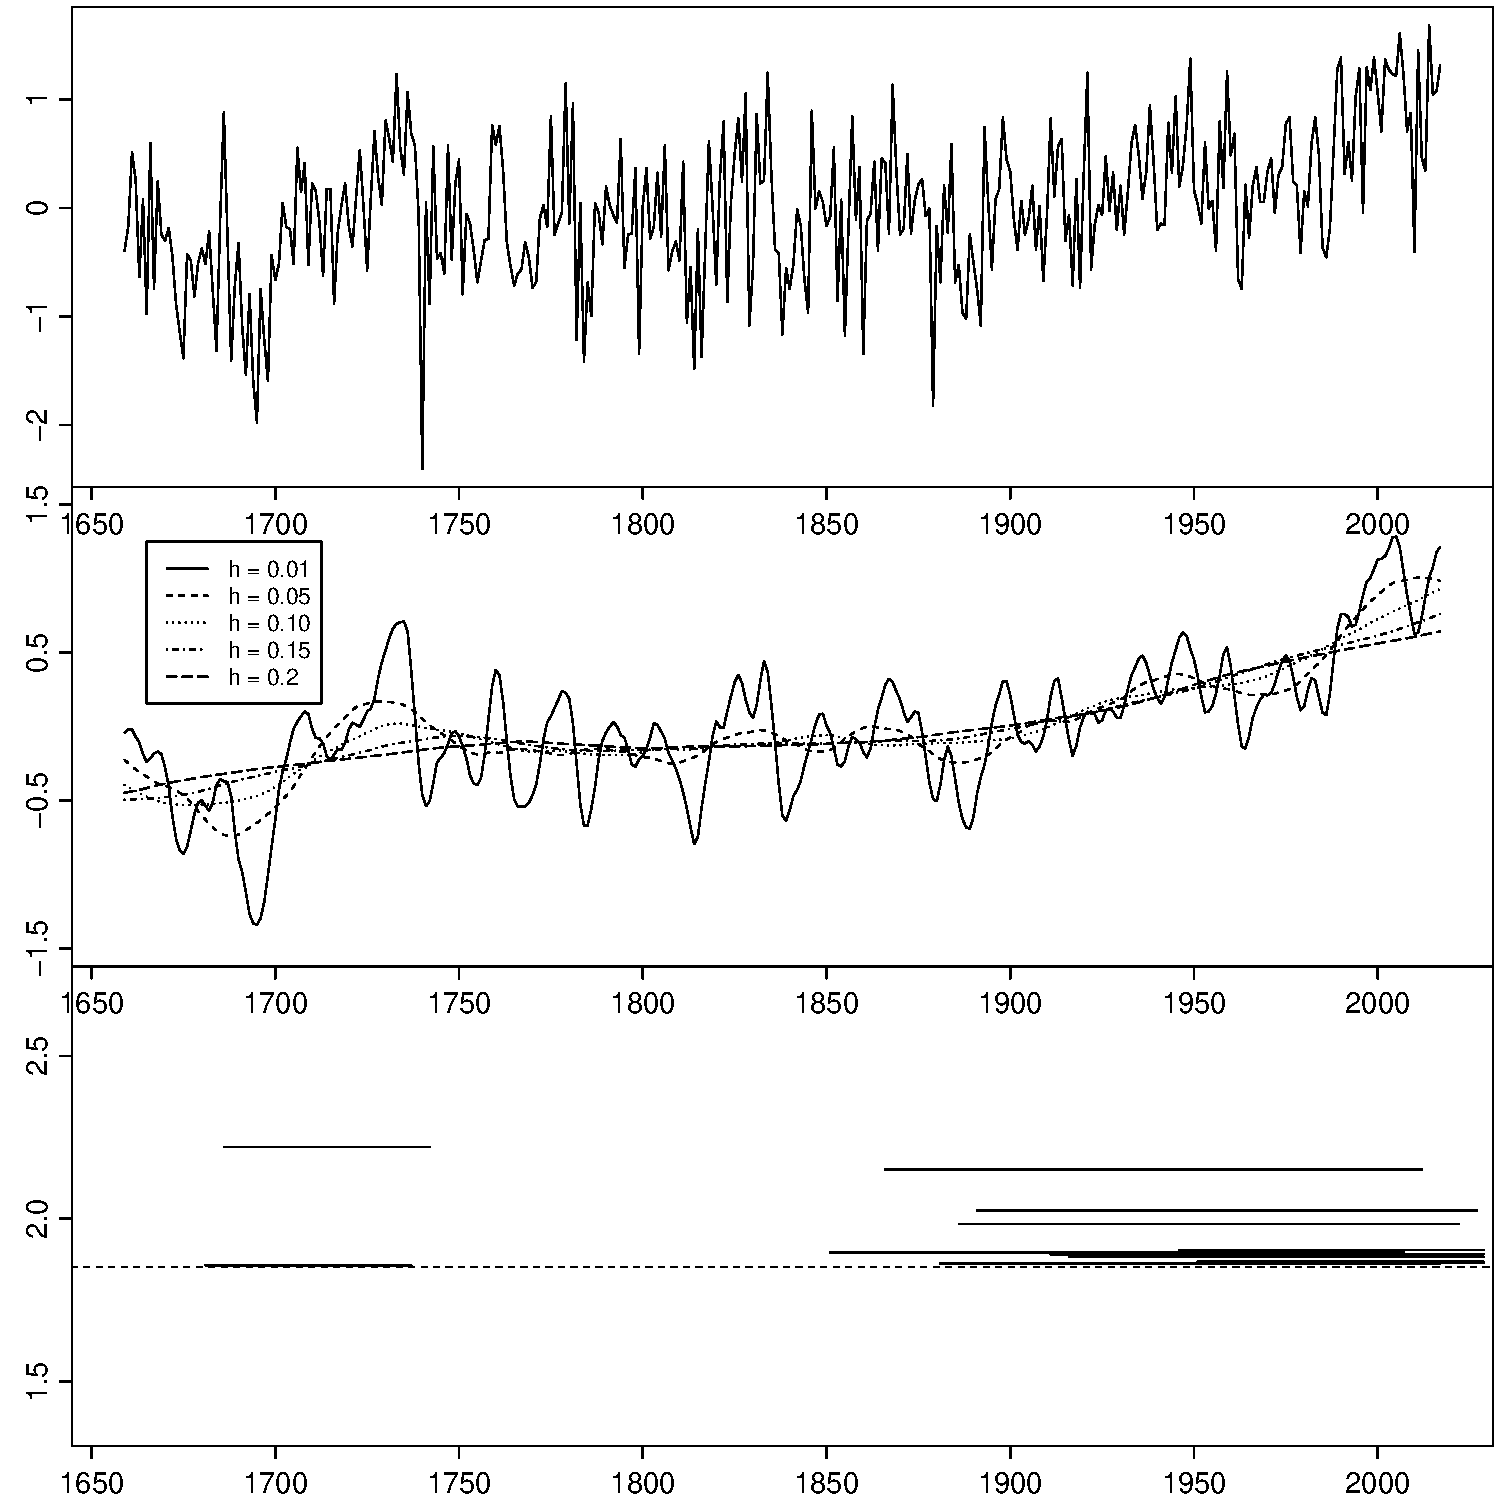
\includepdf[pages=-,pagecommand={},width=\textwidth]{Coding/Output/threegraphics_testing_constant_method_ll.pdf}
\caption{Yearly temperature data for England\label{yearly_data}}
\end{figure}

